%%%%%%%%%%%%%%%%%%%%%%%%%%%%%%%%%%%%%%%%%
% Beamer Presentation
% LaTeX Template
% Version 1.0 (10/11/12)
%
% This template has been downloaded from:
% http://www.LaTeXTemplates.com
%
% License:
% CC BY-NC-SA 3.0 (http://creativecommons.org/licenses/by-nc-sa/3.0/)
%
%%%%%%%%%%%%%%%%%%%%%%%%%%%%%%%%%%%%%%%%%

%----------------------------------------------------------------------------------------
%	PACKAGES AND THEMES
%----------------------------------------------------------------------------------------

\documentclass{beamer}

\mode<presentation> {

% The Beamer class comes with a number of default slide themes
% which change the colors and layouts of slides. Below this is a list
% of all the themes, uncomment each in turn to see what they look like.

%\usetheme{default}
%\usetheme{AnnArbor}
%\usetheme{Antibes}
%\usetheme{Bergen}
%\usetheme{Berkeley}
%\usetheme{Berlin}
%\usetheme{Boadilla}
%\usetheme{CambridgeUS}
%\usetheme{Copenhagen}
%\usetheme{Darmstadt}
%\usetheme{Dresden}
%\usetheme{Frankfurt}
%\usetheme{Goettingen}
%\usetheme{Hannover}
%\usetheme{Ilmenau}
%\usetheme{JuanLesPins}
%\usetheme{Luebeck}
\usetheme{Madrid}
%\usetheme{Malmoe}
%\usetheme{Marburg}
%\usetheme{Montpellier}
%\usetheme{PaloAlto}
%\usetheme{Pittsburgh}
%\usetheme{Rochester}
%\usetheme{Singapore}
%\usetheme{Szeged}
%\usetheme{Warsaw}

% As well as themes, the Beamer class has a number of color themes
% for any slide theme. Uncomment each of these in turn to see how it
% changes the colors of your current slide theme.

%\usecolortheme{albatross}
%\usecolortheme{beaver}
%\usecolortheme{beetle}
%\usecolortheme{crane}
%\usecolortheme{dolphin}
%\usecolortheme{dove}
%\usecolortheme{fly}
%\usecolortheme{lily}
%\usecolortheme{orchid}
%\usecolortheme{rose}
%\usecolortheme{seagull}
%\usecolortheme{seahorse}
%\usecolortheme{whale}
%\usecolortheme{wolverine}

%\setbeamertemplate{footline} % To remove the footer line in all slides uncomment this line
\setbeamertemplate{footline}[page number] % To replace the footer line in all slides with a simple slide count uncomment this line

\setbeamertemplate{navigation symbols}{} % To remove the navigation symbols from the bottom of all slides uncomment this line
}

\usepackage{graphicx} % Allows including images
\usepackage{booktabs} % Allows the use of \toprule, \midrule and \bottomrule in tables
%\usepackage {tikz}
\usepackage{tkz-graph}
\GraphInit[vstyle = Shade]
\tikzset{
  LabelStyle/.style = { rectangle, rounded corners, draw,
                        minimum width = 2em, fill = yellow!50,
                        text = red, font = \bfseries },
  VertexStyle/.append style = { inner sep=5pt,
                                font = \normalsize\bfseries},
  EdgeStyle/.append style = {->, bend left} }
\usetikzlibrary {positioning}
%\usepackage {xcolor}
\definecolor {processblue}{cmyk}{0.96,0,0,0}
%----------------------------------------------------------------------------------------
%	TITLE PAGE
%----------------------------------------------------------------------------------------

\title[Short title]{SimpleMessenger with Apache Thrift} % The short title appears at the bottom of every slide, the full title is only on the title page

\author{Animesh Baranawal} % Your name
% \institute[UC Riverside] % Your institution as it will appear on the bottom of every slide, may be shorthand to save space
%{
%University of California \\ % Your institution for the title page
%\medskip
%}
\date{\today} % Date, can be changed to a custom date

\begin{document}

\begin{frame}
\titlepage % Print the title page as the first slide
\end{frame}

\begin{frame}
\frametitle{Overview} % Table of contents slide, comment this block out to remove it
\tableofcontents % Throughout your presentation, if you choose to use \section{} and \subsection{} commands, these will automatically be printed on this slide as an overview of your presentation
\end{frame}

%----------------------------------------------------------------------------------------
%	PRESENTATION SLIDES
%----------------------------------------------------------------------------------------

%------------------------------------------------

\section{Backend}
\begin{frame}{Data Structures in Thrift}
    \begin{itemize}
        \item \textbf{UserDefinition}: string uniqueID, string ip\_addr, i32 port
        \item \textbf{GroupDefinition}: string groupID, list\texttt{<}string\texttt{>} members
        \item \textbf{Message}: i64 timestamp, string msgString, string toID, string fromID, bool multicast
        \item \textbf{FileDefinition}: binary data, string fileID, i32 size
        \item \textbf{FileChunk}: binary data, i32 size, i32 offset
    \end{itemize}
\end{frame}
\begin{frame}{Services in Thrift}
\begin{itemize}
    \item \textbf{ServerService}: RPC methods: \textit{join}, \textit{connectTo}, \textit{sendMessage}, \textit{joinGroup}, \textit{leaveGroup}
    \item \textbf{FileTransferService}: RPC methods: \textit{startUpload}, \textit{uploadChunk}, \textit{endUpload}, \textit{startDownload}, \textit{downloadChunk}
    \item \textbf{ClientService}: RPC methods: \textit{receive}
\end{itemize}
\end{frame}
\section{Workflows}
\begin{frame}{Messaging Workflow}
\begin{figure}[h]
    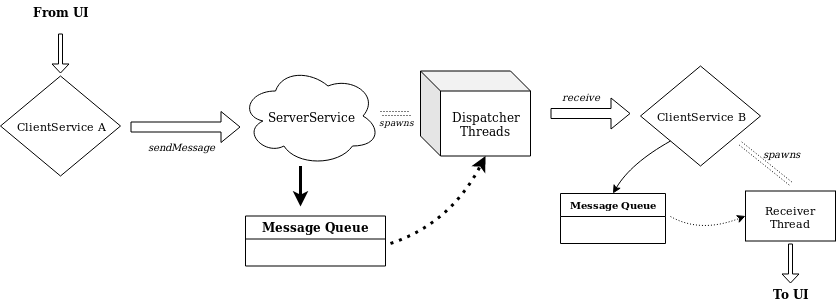
\includegraphics[scale=0.4]{messageWorkflow}
    \caption{Visual description of messaging workflow}
    \label{fig:diagram1}
\end{figure}
\end{frame}
\begin{frame}{File Transfer Workflow}
\begin{figure}[h]
    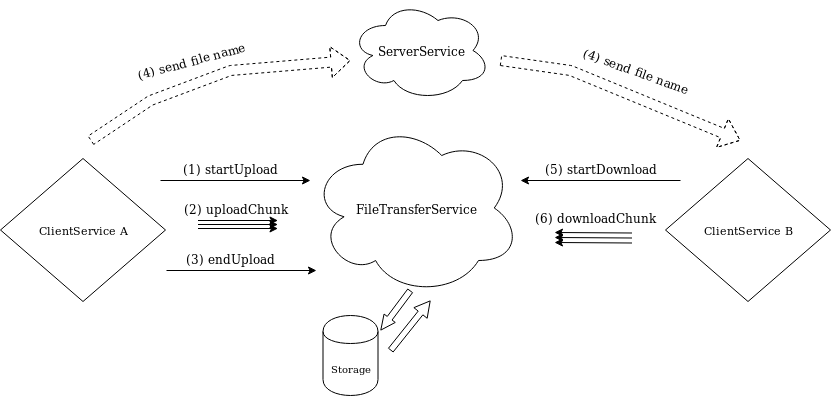
\includegraphics[scale=0.35]{FileTransferWorkflow}
    \caption{Visual description of file transfer workflow}
    \label{fig:diagram2}
\end{figure}
\end{frame}
\section{Results}
\begin{frame}{Latency Observations}
\begin{figure}[!h]
\hspace{-2cm}
\begin{minipage}[t]{5cm}
    \centering
	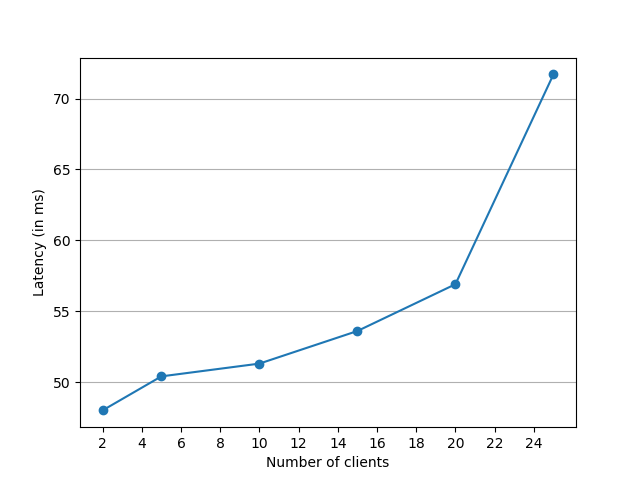
\includegraphics[scale=0.35]{P2P_t1}
	\caption{P2P Latency}
	\label{fig:Diagram3}
\end{minipage}
\hspace{0.5cm}
\begin{minipage}[t]{5cm}
    \centering
	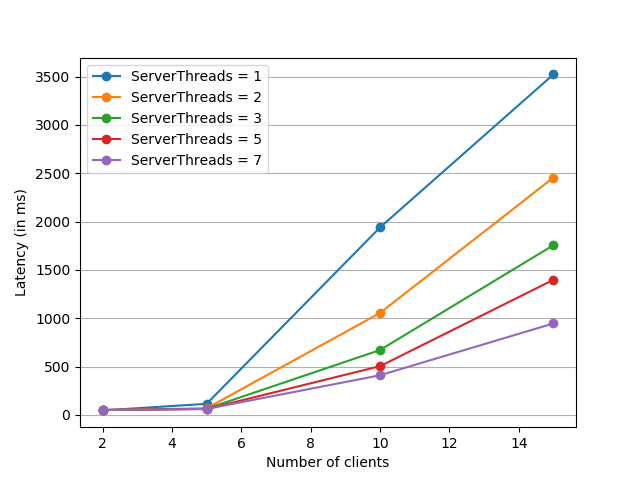
\includegraphics[scale=0.35]{Room_tAll}
	\caption{Multicast Latency}
	\label{fig:Diagram4}
\end{minipage}
\end{figure}
\end{frame}
\begin{frame}{File Transfer Time Observations}
\begin{figure}[h]   
    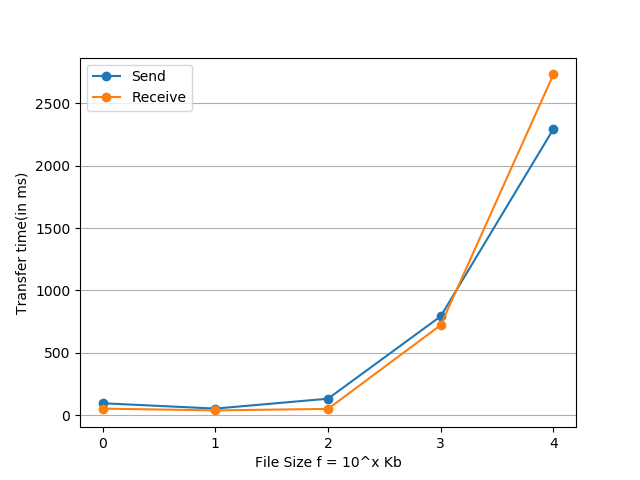
\includegraphics[scale=0.5]{fileTransfer_5Readings}
    \caption{File transfer time for different file sizes}
    \label{fig:diagram2}
\end{figure}
\end{frame}
\end{document}